\documentclass[12pt,a4paper]{article}
\usepackage[pdftex]{graphicx}
\graphicspath{{Image/}}
\usepackage{epstopdf}
\usepackage{float}
\usepackage{amsmath}
\usepackage{mathtools}
\DeclarePairedDelimiter\abs{\lvert}{\rvert}
\DeclarePairedDelimiter\norm{\lVert}{\rVert}
\usepackage{esint}
\usepackage{amsfonts}
\usepackage{times}
\usepackage[top=.4 in, left=0.9in, right=0.9in]{geometry}
\usepackage{bbm}
\usepackage{dsfont}
\usepackage{enumerate}
\usepackage{titlesec}
\newcommand{\rn}{\mathbb{R}}
\newcommand{\E}{\mathbb{E}}
\newcommand{\Gn}{\mathbb{G}_{n}}
\newcommand{\G}{\mathbb{G}}
\newcommand {\tab}{\hspace{10 mm}}
\DeclareMathOperator*{\argmax}{arg\,max}
\DeclareMathOperator*{\argmin}{arg\,min}
\titleformat{\section}[block]{\large \it \filcenter}{}{0.5 ex}{}
\titleformat{\subsection}[block]{\small\it \filcenter}{}{0.5 em}{}
\titleformat{\subsubsection}[block]{\small\it \filcenter}{}{0.5 em}{}
\title{Empirical Methods in Economics\\\small{Assignment VI}\vspace{-9ex}}
\date{Orville D. Mondal\\ $22^{nd}$ of January, 2019\vspace{-3ex}}
\begin{document}
\maketitle
\begin{enumerate}[1.]
\item The firm's dynamic optimisation problem may be stated as the solution to the following Bellman Equation:
\[V(p,x)=\max_{x^\prime\in[0,x]}\left\{p(x-x^\prime)-\frac{1}{5}(x-x^\prime)^{3/2}+\delta\E_{p^\prime\mid p}V(p^\prime,x^\prime)\right\},\text{ where }\]
\[p^\prime=\frac{1}{2}+\frac{1}{2}p+\varepsilon,\hspace{3mm}\varepsilon\sim N(0,0.01);\hspace{3mm} x\in [0,100]; \hspace{3mm} \delta=0.95\]
The state variable is a pair $(p,x)$ corresponding to the price prevailing at a time period, and the stock of `lumber' available to the firm. Prime follows an AR(1) process. The policy variable is the amount of lumber available at the start of the next period. 
\item Using Tauchen's procedure is routine, except that we must specify that the error term is distributed $N(1/2,0.01)$, due to the presence of an additional term in the AR(1) process. The generated grid of prices, and the transition matrix is denoted `grid' and `prob', respectively. 
\item Value function iteration is routine. The only modification made is to the utility function, which is as specified in the assignment for all positive values of lumber harvested. Harvesting more than is available at a given date results in a penalty of -100. This ensures that the value and policy functions calcuated are correct.  
\begin{figure}[h]
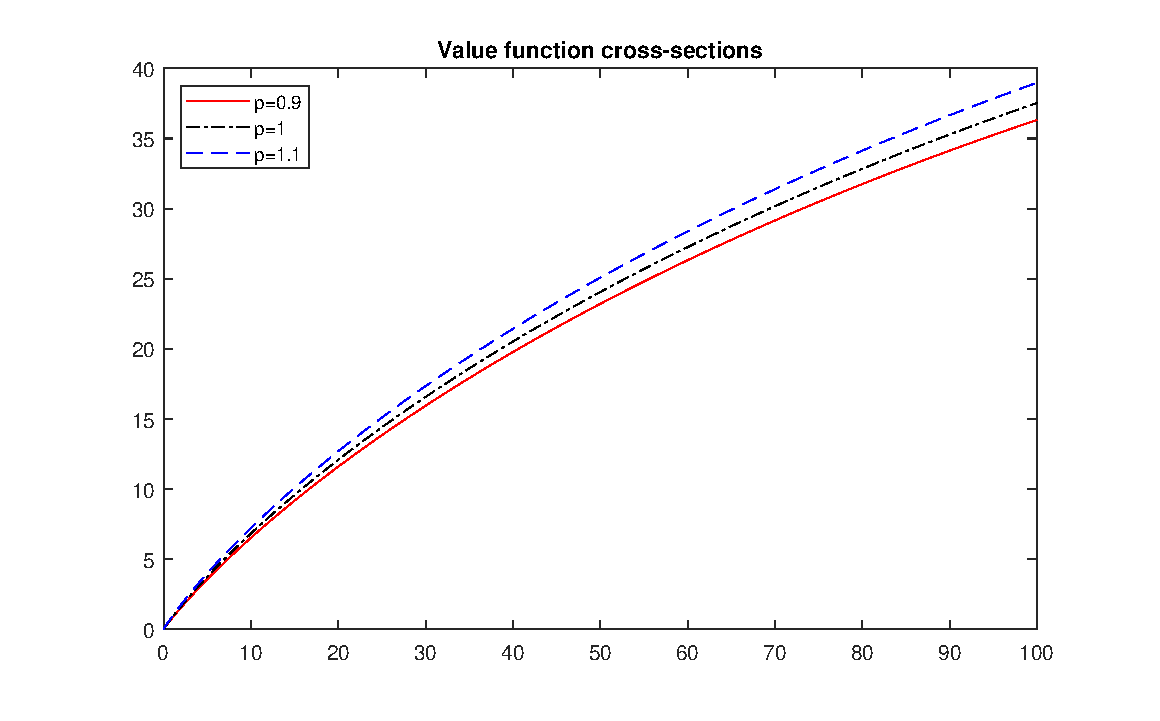
\includegraphics[width=\textwidth]{value.eps}\vspace{-3ex}
\caption{Value function at different price levels.}
\end{figure}
\newgeometry{top=.9 in, left=0.9in, right=0.9in}
\item The following figure plots optimal next period stock, by price for different levels of starting stock. The figure is intuitive: the higher the present price, the more lumber the firm would want ot harvest, to maximise present day profits. \\
NOTE: The y-axis shows optimal stock multiplied by 100, so 200 corresponds to 20 units of stock next period. 

\begin{figure}[h]
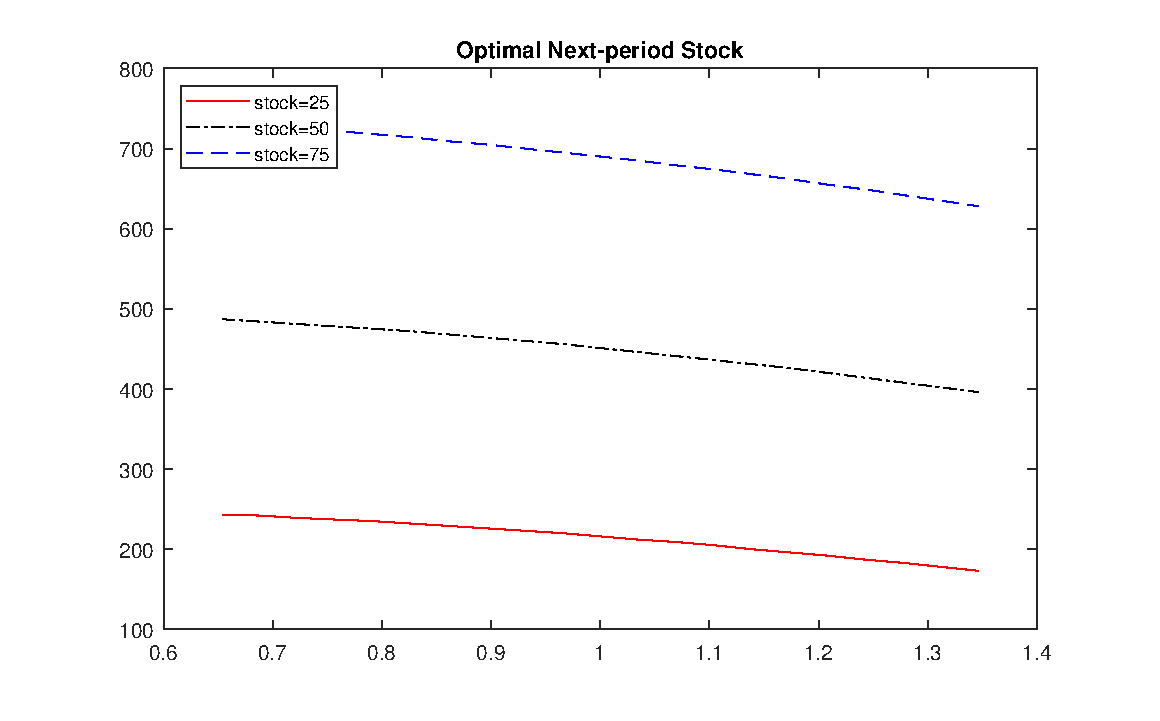
\includegraphics[width=\textwidth]{stock.eps}\vspace{-3ex}
\caption{Optimal stock by price.}
\end{figure}
\item The patterns when using a price grid of 5 points look roughly the same, although the linear interpolation for the policy function is hiding the fact that there are only 5 points on the x-axis. Even the scale of the value functions appears conformable to that when using the 21 point price grid. There appears to be more of a gap between the individual value function lines (corresponding to a particular price), but this is an artifact of the coarse grid because the line for price equalling 0.9 is actually the line for a slightly lower price (the line labelled for price=1.1, actually corresponds to a slightly higher price). The figures are on the next page.
\begin{figure}[h]
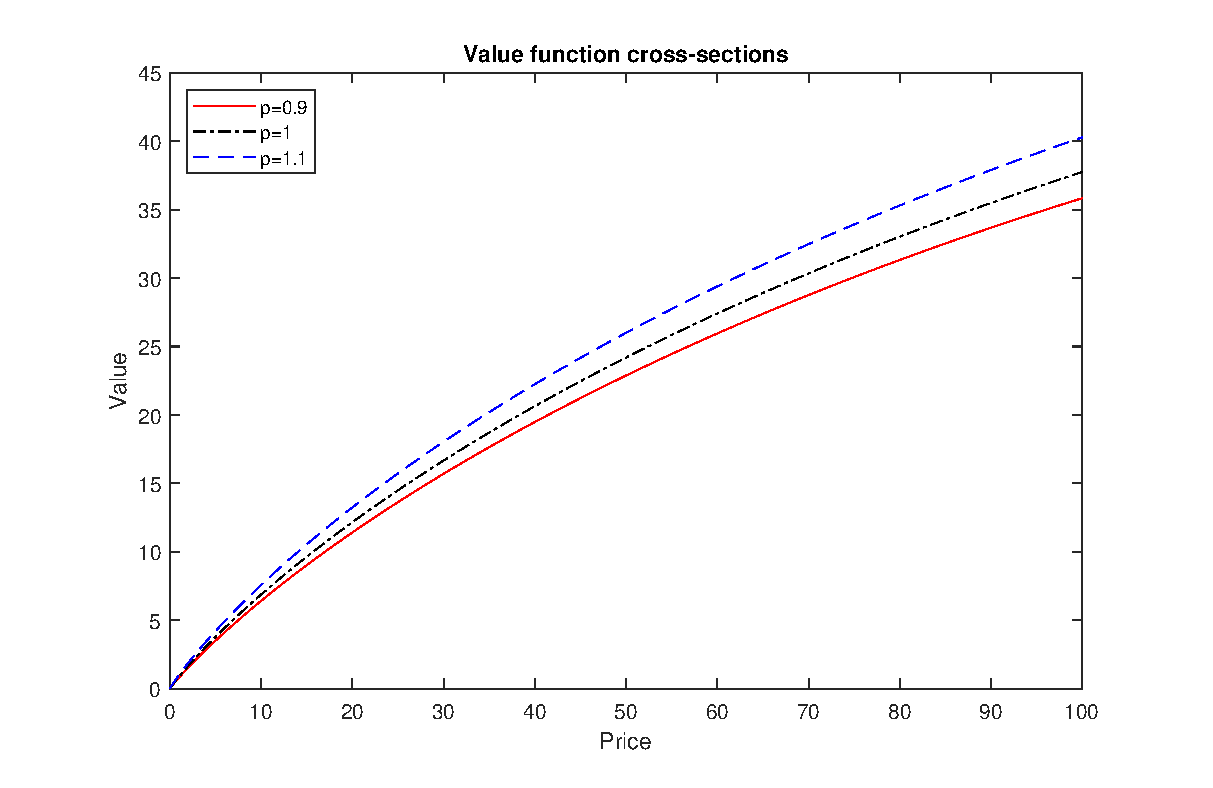
\includegraphics[width=\textwidth]{value2.eps}\vspace{-3ex}
\caption{Value function at different price levels, with coarse price grid.}
\end{figure}
\begin{figure}[h]
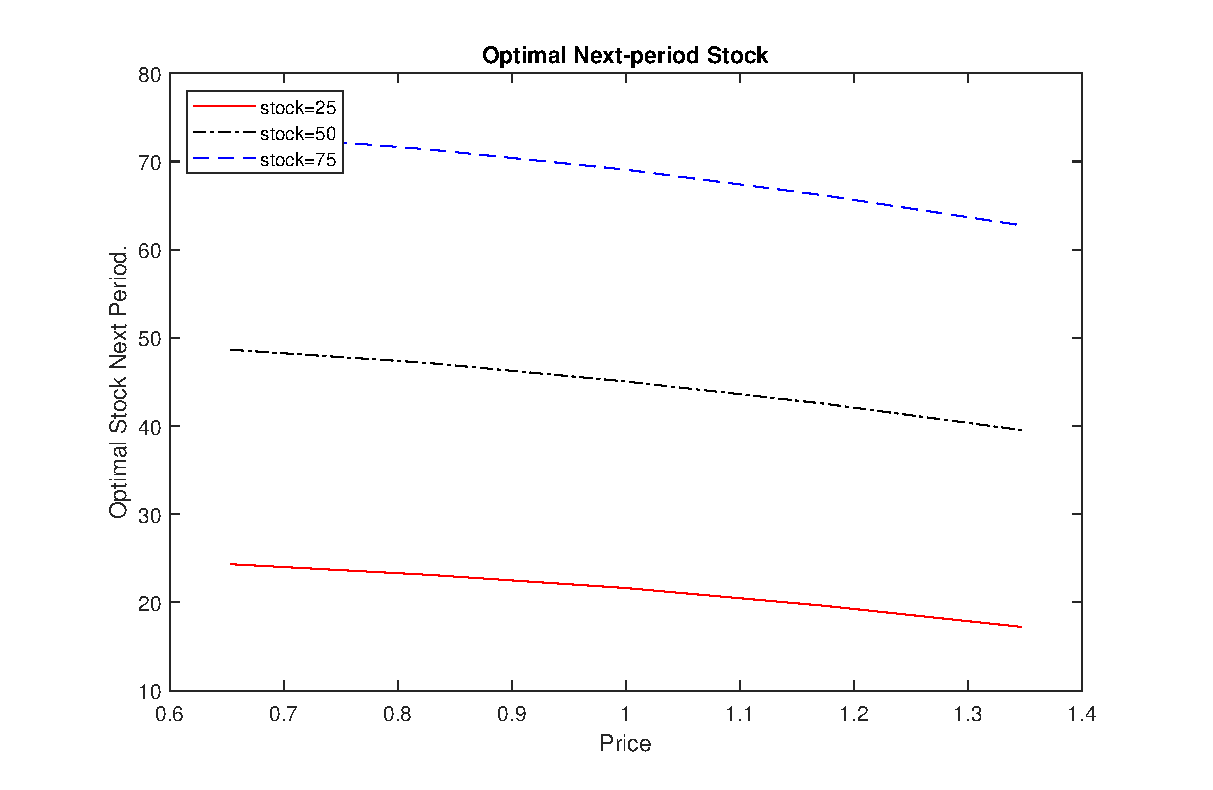
\includegraphics[width=\textwidth]{stock2.eps}\vspace{-3ex}
\caption{Optimal stock by price, on coarse grid.}

\end{figure}
\restoregeometry
\end{enumerate}
\end{document}